\documentclass[UTF8,a4paper,11pt,fontset=fandol]{ctexart}

\usepackage[margin=2.2cm]{geometry}
\usepackage{amsmath,amssymb}
\usepackage{booktabs}
\usepackage{graphicx}
\usepackage{hyperref}
\usepackage{tikz}
\ctexset{
  section = {
    format = \Large\bfseries\raggedright
  }
}
\usetikzlibrary{arrows.meta,positioning}

\hypersetup{hidelinks}
\graphicspath{{figures/}}
\linespread{1.18}
\emergencystretch=2em

\title{\heiti 基于视觉特征对比的模拟 K 线图涨跌分类研究}
\author{23089056孙琉屿、23089057张伟杰、23089058王显辰}
\date{}

\begin{document}
% \ctexset{
%   section = {
%     format = \Large\bfseries\raggedright
%   }
% }
\maketitle

\begin{abstract}
K 线图把金融时间序列转化为带有颜色、边缘和相对位置关系的二维图像，因此可以作为计算机视觉方法进入金融分析场景的一个小切口。本文围绕“给定一段 K 线图，判断后续短期价格方向”这一二分类任务，构建了一个可复现实验：先模拟具有趋势持续性的 OHLC 价格序列，再将 30 个交易日窗口渲染为 $96\times96$ 的 K 线图，并比较多数类基线、原始灰度像素 + 线性 SVM、HOG + 线性 SVM 以及 HOG 与图像统计线索融合的分类效果。在 1200 个模拟样本上，原始灰度像素 + SVM 在 300 个测试样本中取得 82.67\% 的准确率和 81.94\% 的 F1 值，优于多数类基线的 52.00\% 准确率，也略高于 HOG 特征。实验说明，在受控模拟环境下，K 线图中的整体形态确实包含可被视觉分类器学习的方向信号；但由于本文没有使用真实市场数据，结果只能说明流程可行性，不能直接解释为实际交易收益。
\end{abstract}

\noindent\textbf{关键词：}计算机视觉；K 线图；图像分类；HOG；支持向量机；金融图像

\section{引言}

股票、指数和期货价格通常以时间序列形式存储，但交易者阅读市场时经常借助 K 线图。K 线图把开盘价、最高价、最低价和收盘价压缩到一个小的视觉符号中，连续 K 线又形成了颜色交替、影线长短和价格斜率等图像模式。这种表示使金融预测问题带有视觉属性：如果一段价格序列的局部形态与后续走势存在统计关系，那么图像分类器也许能够从图像中展现这种关系。

K 线图涨跌分类符合财经视觉任务的要求，输入、输出和评价指标都比较清楚，且不依赖复杂标注，可以用程序生成数据和图像，便于在课程作业环境中完整复现实验。因此，本文选择 K 线图涨跌分类作为选题。当然，模拟数据也带来明显边界：它能帮助验证“时间序列转图像后能否被视觉特征分类”这个流程，却不能替代真实市场数据上的交易回测。

本文完成了三方面工作：构建了一个从模拟 OHLC 序列到 K 线图像的可复现数据流程；比较了原始像素、HOG 以及融合颜色和几何统计线索的视觉特征；通过准确率、精确率、召回率、F1 值和混淆矩阵分析不同特征对涨跌分类的影响。

\section{相关工作}

将金融时间序列转化为图像并用视觉模型学习，是近年来金融机器学习中的一个重要思路。Sezer 和 {\"O}zbayo{\u{g}}lu 将多个技术指标转化为二维图像，并使用深度卷积网络进行算法交易实验，说明二维图像表示可以为金融预测提供不同于手工指标的特征空间 \cite{sezer2018trading}。Jiang、Kelly 和 Xiu 进一步使用股票价格图像研究趋势可预测性，强调机器学习图像分析能够从价格图中提取传统动量或反转信号之外的形态 \cite{jiang2023price}。这些研究使用真实市场数据和更大规模模型，而本文更关注课程作业场景下的最小可复现实验，因此采用模拟 K 线图与线性分类器来展示基本流程。

在视觉特征方面，Dalal 和 Triggs 提出的方向梯度直方图（Histogram of Oriented Gradients, HOG）通过统计局部梯度方向描述物体轮廓，在行人检测等任务中具有代表性 \cite{dalal2005hog}。K 线图虽然不是自然图像，但蜡烛实体、影线和整体斜率也会形成明显边缘，因此 HOG 可作为一个可解释的传统视觉特征。分类器方面，支持向量机通过最大间隔思想学习二分类决策边界，是小规模特征实验中常用且稳定的基线方法 \cite{cortes1995svm}。本文实验代码主要使用 scikit-image 提取 HOG 特征 \cite{vanderwalt2014skimage}，并使用 scikit-learn 训练线性 SVM \cite{pedregosa2011sklearn}。

\section{任务定义与数据生成}

本文研究的输入是一张由连续 30 个交易日 OHLC 数据渲染得到的 K 线图，输出是未来 5 个交易日的二分类方向标签。对第 $i$ 个样本，设历史窗口为
\[
S_i=\{(o_t,h_t,l_t,c_t)\}_{t=1}^{30},
\]
其中 $o_t,h_t,l_t,c_t$ 分别表示第 $t$ 日开盘价、最高价、最低价和收盘价。未来收益定义为
\[
r_i^{(5)}=\frac{c_{35}}{c_{30}}-1,
\]
标签定义为
\[
y_i=\mathbb{I}(r_i^{(5)}>0).
\]
当 $y_i=1$ 时样本属于“上涨”类，否则属于“下跌”类。分类器只能看到前 30 日生成的图像，未来 5 日价格只用于产生标签。

由于当前目录中没有真实股票数据集，本文使用可控的模拟过程生成 OHLC 序列。每个样本先随机选择一个上涨或下跌趋势方向，再用带漂移项的随机收益过程生成价格路径。默认参数中，样本数为 1200，历史窗口长度为 30，预测跨度为 5，图像大小为 $96\times96$，随机种子为 42。渲染时，上涨蜡烛使用绿色、下跌蜡烛使用红色，影线使用深灰色，价格范围按每个窗口的最高价和最低价归一化到图像坐标。图 \ref{fig:samples} 展示了部分生成样本，可以看到上涨类和下跌类在整体走势上存在可见差异，同时局部波动仍会制造一定混淆。

\begin{figure}[htbp]
  \centering
  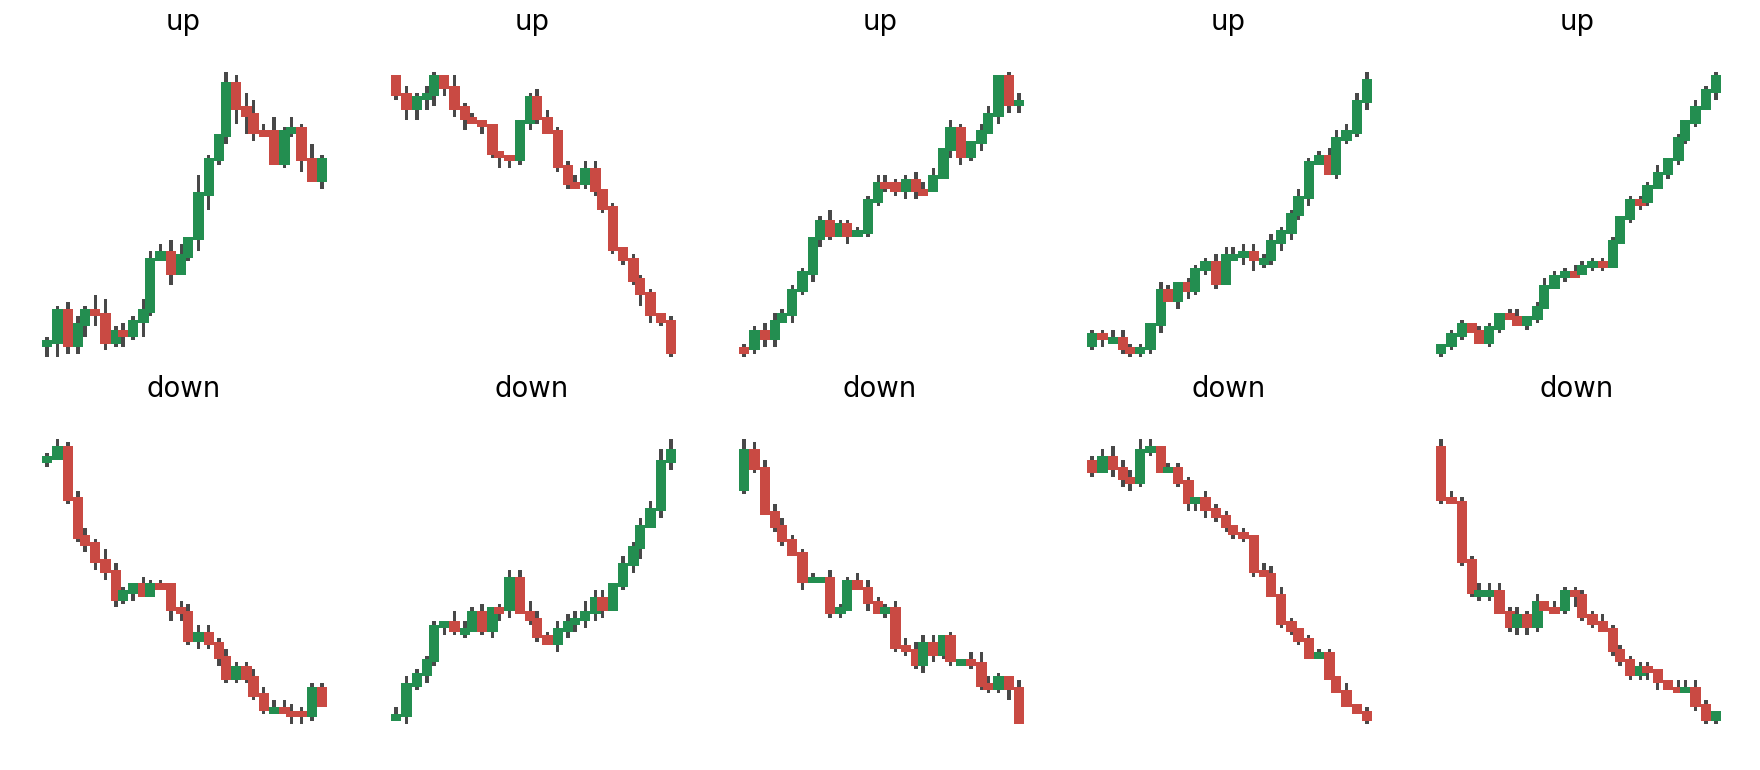
\includegraphics[width=0.95\linewidth]{sample_candlesticks.png}
  \caption{模拟 K 线图样本。图像上方标注为未来 5 日方向标签，分类器输入仅包含当前 30 日窗口。}
  \label{fig:samples}
\end{figure}

\section{方法}

本文方法流程如图 \ref{fig:pipeline} 所示。首先生成模拟 OHLC 序列并渲染为 K 线图像，然后分别抽取原始像素特征、HOG 特征和融合特征，最后用线性 SVM 完成二分类。这样的设计有意保持简单：它不依赖预训练网络，也不需要外部数据下载，便于复现并分析每一种视觉表示到底贡献了什么。

\begin{figure}[htbp]
  \centering
  \begin{tikzpicture}[
    node distance=1.15cm,
    box/.style={draw, rounded corners=2pt, align=center, minimum width=2.8cm, minimum height=0.85cm},
    arrow/.style={-{Latex[length=2mm]}, thick}
  ]
    \node[box] (ohlc) {模拟 OHLC\\价格窗口};
    \node[box, right=of ohlc] (render) {K 线图\\渲染};
    \node[box, right=of render] (feature) {视觉特征\\提取};
    \node[box, right=of feature] (svm) {线性 SVM\\涨跌分类};
    \draw[arrow] (ohlc) -- (render);
    \draw[arrow] (render) -- (feature);
    \draw[arrow] (feature) -- (svm);
  \end{tikzpicture}
  \caption{本文实验流程。未来收益只参与标签生成，不输入分类器。}
  \label{fig:pipeline}
\end{figure}

原始像素特征先将彩色 K 线图转为灰度图，再将 $96\times96$ 像素矩阵展平为向量：
\[
\phi_{\mathrm{pix}}(I)=\mathrm{vec}(\mathrm{gray}(I)).
\]
这种表示几乎不做先验假设，保留了图像中的全局走势位置和蜡烛排列，但维度较高，也可能对渲染方式敏感。

HOG 特征则更强调局部边缘方向。本文将图像转为灰度后，以 $8\times8$ 像素为 cell、$2\times2$ cell 为 block，统计 9 个方向的梯度直方图。对于 K 线图而言，HOG 可以描述影线和实体边缘形成的局部结构，但它不一定能完整保留“后半段价格整体高于前半段”这类低频趋势信息。

融合特征在 HOG 之外加入少量从图像直接计算的统计线索，包括红绿蜡烛像素占比、不同横向区域的颜色差异、墨迹像素中心线斜率以及首尾区域垂直中心差。融合向量写作
\[
\phi_{\mathrm{fuse}}(I)=[\phi_{\mathrm{hog}}(I),\phi_{\mathrm{cue}}(I)].
\]
这些线索仍然来自渲染后的图像，而不是直接读取原始 OHLC 数值，因此保留了视觉分类任务的设定。

三类特征都输入线性 SVM。令训练标签转换为 $\tilde{y}_i\in\{-1,1\}$，分类器优化目标可写为
\[
\min_{\mathbf{w},b}\frac{1}{2}\|\mathbf{w}\|_2^2
+C\sum_i \max(0,1-\tilde{y}_i(\mathbf{w}^{\top}\phi(I_i)+b)).
\]
实验中所有特征在训练前经过标准化处理，并使用相同的训练集和测试集划分。

\section{实验与结果}

实验使用 1200 个模拟样本，其中 900 个用于训练，300 个用于测试，划分时保持类别比例近似一致。整体上涨样本比例为 48.08\%，因此多数类基线会把所有样本预测为下跌。评价指标包括准确率、精确率、召回率和 F1 值。为了避免偶然性，代码固定随机种子为 42；完整实验脚本位于 \texttt{src/run\_experiment.py}，结果文件位于 \texttt{results/metrics.json}。

\begin{table}[htbp]
  \centering
  \caption{不同视觉特征在模拟 K 线图涨跌分类任务上的结果}
  \label{tab:results}
  \begin{tabular}{lcccc}
    \toprule
    方法 & 准确率 & 精确率 & 召回率 & F1 值 \\
    \midrule
    多数类基线 & 0.5200 & 0.0000 & 0.0000 & 0.0000 \\
    原始灰度像素 + SVM & \textbf{0.8267} & \textbf{0.8194} & \textbf{0.8194} & \textbf{0.8194} \\
    HOG + SVM & 0.8100 & 0.8175 & 0.7778 & 0.7972 \\
    HOG + 图像统计线索 + SVM & 0.8067 & 0.8162 & 0.7708 & 0.7929 \\
    \bottomrule
  \end{tabular}
\end{table}

从表 \ref{tab:results} 可以看到，三种视觉模型都显著高于多数类基线，说明模拟 K 线图中确实存在可以被分类器捕捉的形态信号。原始灰度像素 + SVM 的表现最好，准确率达到 82.67\%，F1 值为 81.94\%。这一结果并不意味着原始像素在真实金融任务中一定优于更复杂特征，而是说明在本文的简洁渲染条件下，价格走势的全局位置关系非常重要，直接展平像素反而完整保留了这些低频信息。

HOG + SVM 的准确率为 81.00\%，低于原始像素约 1.67 个百分点。它仍然明显优于基线，说明蜡烛边缘和局部方向对分类有帮助；但 HOG 更擅长描述局部形状，对整体趋势的表达不如像素特征直接。融合颜色和几何统计线索后，结果没有继续提升，可能原因是这些统计量与 HOG 已有信息重叠，且线性 SVM 在当前样本规模下没有从 19 维附加线索中学到更稳定的增益。图 \ref{fig:metric} 给出了准确率和 F1 值的柱状比较。

\begin{figure}[htbp]
  \centering
  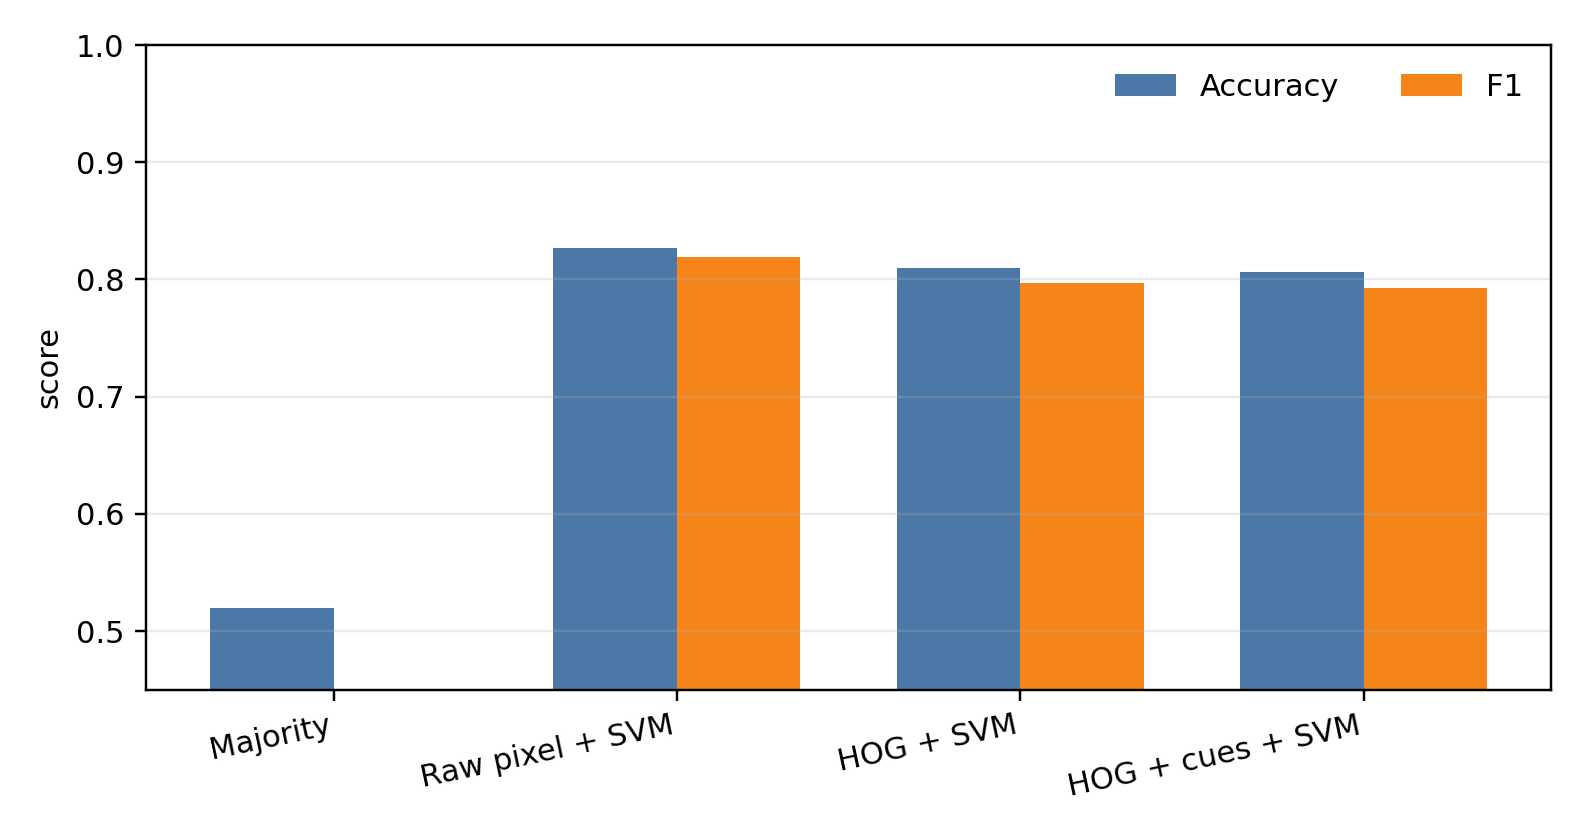
\includegraphics[width=0.76\linewidth]{metric_comparison.png}
  \caption{不同方法的准确率与 F1 值比较。}
  \label{fig:metric}
\end{figure}

最佳模型的混淆矩阵如图 \ref{fig:cm} 所示。在 156 个真实下跌样本中，模型正确识别 130 个；在 144 个真实上涨样本中，模型正确识别 118 个。上下两类的错误数量相同，说明模型没有表现出明显偏向某一类的倾向。结合样本图可以推测，错误多出现在历史窗口走势先涨后跌或先跌后涨的样本中，这类图像的局部形态与未来标签之间并不完全一致。

\begin{figure}[htbp]
  \centering
  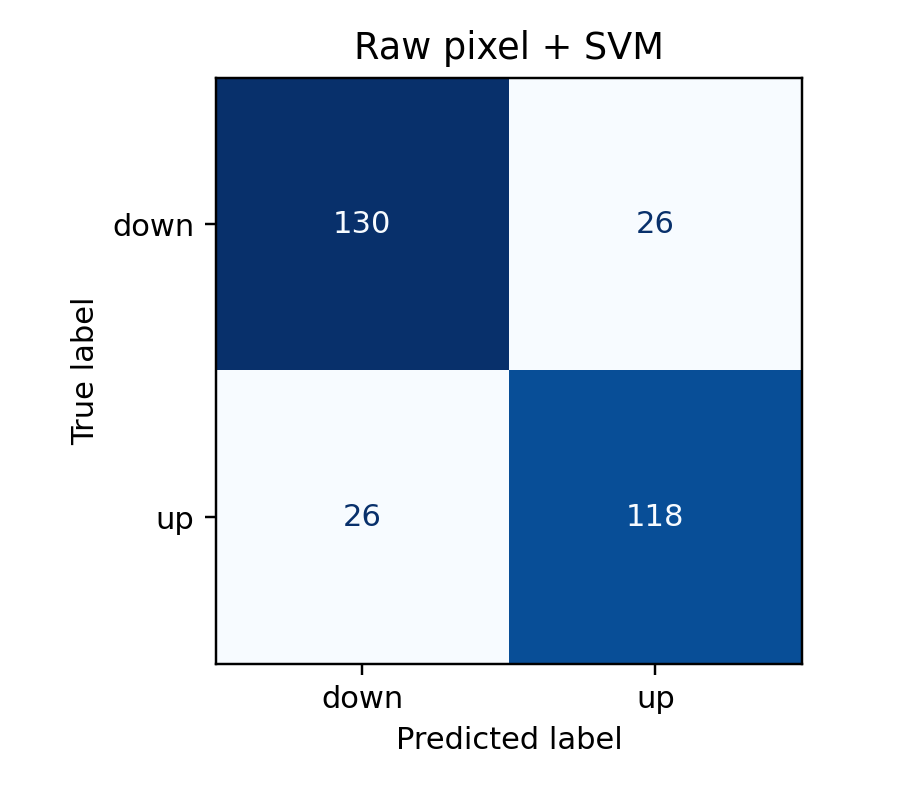
\includegraphics[width=0.48\linewidth]{confusion_matrix.png}
  \caption{最佳模型“原始灰度像素 + SVM”的测试集混淆矩阵。}
  \label{fig:cm}
\end{figure}

\section{结论}

本文以模拟 K 线图为输入，定义未来 5 日涨跌分类任务，并比较了多种简单视觉特征与线性 SVM 的组合。实验结果表明，在带有趋势持续性的受控模拟数据上，视觉模型能够明显优于多数类基线，其中原始灰度像素 + SVM 取得了 82.67\% 的准确率和 81.94\% 的 F1 值。这个结果支持了一个朴素但重要的结论：当时间序列被稳定地渲染为图像后，图像中的空间形态可以承载可学习的方向信息。

本文也存在明显局限。首先，数据来自模拟过程，标签与图像之间的统计关系由生成机制决定，因此结果不能直接推广到真实股票、指数或期货市场。其次，本文只使用线性 SVM 和传统视觉特征，没有比较卷积神经网络、Transformer 或多模态方法。未来工作可以引入真实历史行情数据，按时间顺序划分训练集和测试集，并进一步比较 ResNet、轻量级 CNN 与本文传统特征方法之间的差异。若面向真实交易应用，还需要加入交易成本、滑点和风险控制等评估，而不仅仅报告分类准确率。

\section*{分工说明}

王显辰（23089058）负责选题设计与相关工作整理；孙琉屿（23089056） 负责实验代码、数据生成和图表绘制；张伟杰（23089057）负责论文撰写、排版和最终复核。

\bibliographystyle{unsrt}
\bibliography{references}

\end{document}
